% Path diagram of the linear growth curve model (vignette lin-growth).
\documentclass[tikz, border = 6pt]{standalone}
\usepackage{amsmath}
\usepackage{bm}
\usetikzlibrary{arrows.meta, positioning, calc}
\tikzset{
  lat/.style = {circle, draw, thick, minimum size = 12mm, inner sep = 0pt},
  obs/.style = {rectangle, draw, thick, minimum size = 10mm, inner sep = 1pt},
  noise/.style = {circle, draw, minimum size = 7mm, inner sep = 0pt},
  reg/.style = {-{Stealth[length = 2.5mm]}, thick},
  cov/.style = {{Stealth[length = 2mm]}-{Stealth[length = 2mm]}},
  var/.style = {cov, looseness = 5},
  lab/.style = {font = \footnotesize, fill = white, inner sep = 1pt},
  dots/.style = {font = \Large}
}
\begin{document}
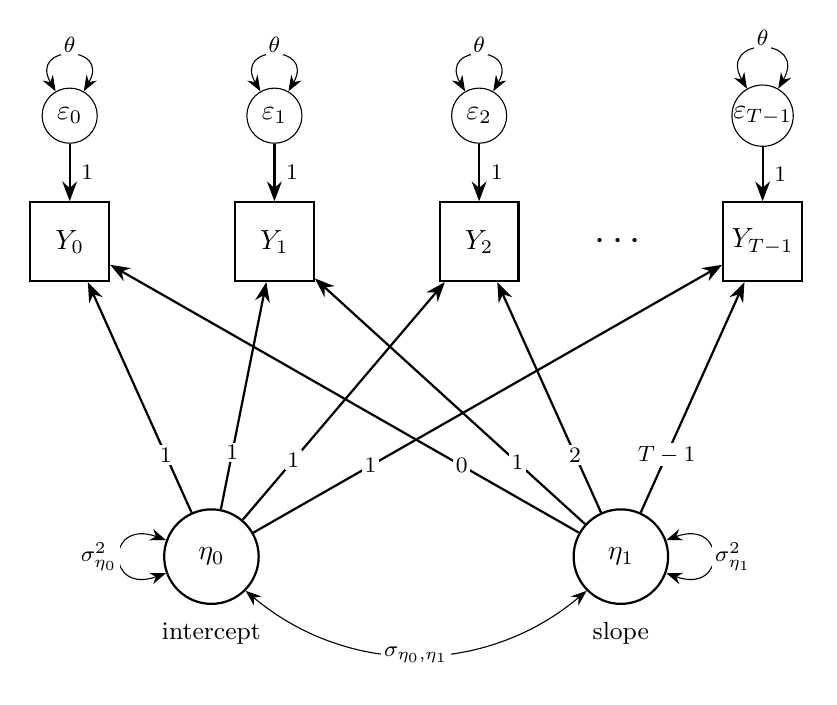
\begin{tikzpicture}
  % occasions
  \foreach \t/\x/\l in {1/0/0, 2/2.6/1, 3/5.2/2, T/8.8/T - 1} {
    \node[obs] (y\t) at (\x, 0) {$Y_{\l}$};
    \node[noise] (u\t) at (\x, 1.6) {$\varepsilon_{\l}$};
    \draw[reg] (u\t) -- node[lab, right = 1mm] {1} (y\t);
    % residual variance
    \draw[var] (u\t.60) to[out = 60, in = 120]
      node[lab, above] {$\theta$} (u\t.120);
  }
  \node[dots] at (7, 0) {$\cdots$};
  % intercept and slope
  \node[lat] (i) at (1.8, -4) {$\eta_{0}$};
  \node[lat] (s) at (7, -4) {$\eta_{1}$};
  \node[font = \small, below = 1mm of i] {intercept};
  \node[font = \small, below = 1mm of s] {slope};
  \foreach \t in {1, 2, 3, T} {
    \draw[reg] (i) -- node[lab, pos = 0.25] {1} (y\t);
  }
  \foreach \t/\l in {1/0, 2/1, 3/2, T/T - 1} {
    \draw[reg] (s) -- node[lab, pos = 0.25] {$\l$} (y\t);
  }
  % intercept and slope variances
  \draw[var] (i.160) to[out = 160, in = 200]
    node[lab, left] {$\sigma^{2}_{\eta_{0}}$} (i.200);
  \draw[var] (s.20) to[out = 20, in = -20]
    node[lab, right] {$\sigma^{2}_{\eta_{1}}$} (s.-20);
  % intercept-slope covariance
  \draw[cov] (i.south east) to[out = -40, in = 220]
    node[lab] {$\sigma_{\eta_{0}, \eta_{1}}$} (s.south west);
\end{tikzpicture}
\end{document}